\section{Selection}
\label{sec:selection}

\sean{Move to intro from here--}
Current implementations of crowdsourcing in databases such as CrowdDB \cite{DBLP:conf/sigmod/FranklinKKRX11} and Qurk \cite{DBLP:conf/sigmod/MarcusWKMM11} have focused primarily on using human computation at the query processing level, enabling human workers to fill in missing tables when the data is queried.  The query itself allocates on-line which entries should be modified by humans.  \sysName contrasts with this methodology by pre-processing the crowdsourcing portions off-line.

The problem that results is in which entries should be sent to the crowd for modification.  The underlying data model of \sysName is a database of tokens.  We can represent each token in terms of a question posted to Mechanical Turk.  Such questions provide a token and allow workers to supply the true label of that token.  Given that large scale databases may contain millions of token entries, asking any type of large subset can become prohibitively expensive.  For instance, asking 5 Turkers per question at \$0.01 apiece, 100,000 tokens would still cost \$5,000. Therefore, it would help to limit the number of questions needed to produce a sizeable gain in accuracy of the database.\sean{--to here}

In this section, we discuss some optimizations that seek to minimize the number of questions one needs to ask the crowd.  First we discuss methods to constrain the token space, such as limiting only token per document and clustering similar documents into a single question.  Then we describe how to order the remaining space so that given a fixed budget of questions we can optimize the number of cleaned entries using information theory.  We term the entire selection process InfoSelect and the full algorithm is displayed in Figure~\ref{alg:infoselect}. 

\begin{algorithm}[fillcomment]
\label{alg:infoselect}
\SetKwInOut{Input}{input}\SetKwInOut{Output}{output}
\Input{Full database $T$ of tokens}
\Output{Reduced set $S$ of maximum information tokens}
\BlankLine
Initialize hash map $H$\;
Initialize cluster set $C$\;
\CommentSty{//Retain only max entropy tokens from each citation}\;
\ForEach{$t \in T$}{
	\eIf{$H.$containsKey$(t.$docID$)$}{
		currentToken $\leftarrow$ $H(t.$docID$)$\;
		\If{currentToken.entropy $<$ t.entropy}{
			$H(t.$docID$) \leftarrow t$\;
		}
	}{
		$H(t.$docID$) \leftarrow t$\;
	}
}
\CommentSty{//Cluster tokens with similar properties}\;
Load all tokens in $H$ into queue $Q$\;
\ForEach{$t \in Q$}
{
	\ForEach{cluster $c \in C$}
	{
		\If{$c$.text $=$ $t$.text \&\\
			$c$.label $=$ $t$.label \&\\
			$c$.prevLabel $=$ $t$.prevLabel \&\\
			$c$.postLabel $=$ $t$.postLabel}
			{
				Add $t$ to cluster $c$\;
				$c$.totalEntropy $\leftarrow c$.totalEntropy $+ t$.totalEntropy\;
			}
	}
	\If{$t$ not added to a cluster}
	{
		Initialize new cluster $c$\;
		$c$.text $\leftarrow$ $t$.text\;
		$c$.label $\leftarrow$ $t$.label\;
		$c$.prevLabel $\leftarrow$ $t$.prevLabel\;
		$c$.postLabel $\leftarrow$ $t$.postLabel\;
		Add $c$ to cluster set $C$\;
	}
	
}
SORT clusters $c \in C$ by $c$.totalEntropy\;

\caption{InfoSelect}
\end{algorithm}

\subsection{Basic Entropy-based Algorithm}

The first approach to optimizing the set of questions is to determine which ones give the highest quality information.  The selection problem we encounter can be framed in terms of a \textit{Total Utility Function} (TUF) that quantizes the total uncertainty in the database.  Selecting tokens for labeling by the crowd corresponds to a reduction of the TUF and we seek to select those tokens that do this maximally.  While strictly speaking the TUF can be any function of the probabilistic content of each token, we model our function on the total entropy of the system.  For an individual document, this is the entropy over the space of possible labelings \textbf{s}:
\begin{equation}
H(d^{i}) = \sum_{\textbf{s}}p^{i}(\textbf{s})log(p^{i}(\textbf{s}))
\end{equation}
Since all documents in the database are independent, the total entropy is equivalent to the sum of the entropies of each document $\sum_{i}H(d^{i})$.  For a document of length $N$ in a label space of size $L$ there are $N^{L}$ possible values that $\textbf{s}$ may take, making direct calculation intractable for any nontrivial task.  We can bypass this issue by remembering that absolute values of the system entropy are not needed and we care only about relative changes in response to selecting one token over another.  

We consider our selection problem to be one of partitioning the set of all tokens $T$ into those selected for submission and those not.  Let $X$ be the set of tokens pushed to the crowd and $Y$ be the remaining set of tokens such that $Y = T - X$. For a fixed budget, we seek to select $X$ such that $H(Y|X)$ is minimized.  The equation for conditional entropy states from Section~\ref{sec:uncertainty} states
\begin{equation}
H(Y|X) = H(X,Y) - H(X)
\end{equation}
The first part of the right hand side, $H(X,Y)$, is a constant since $X \cup Y = T$.  Thus minimizing $H(Y|X)$ is equivalent to maximizing $H(X)$, the entropy of the selected tokens.  If selection is done on-line one token at a time, $H(X)$ is the marginal entropy of an individual token and top-k selection is equivalent to selecting the top-k marginal entropies from $T$.  Explicitly, the marginal entropy for token $i$ is:

\begin{equation}
H^{i} = -\sum^{L}_{j=1}p^{i}_{j}log(p^{i}_{j})
\end{equation}

\begin{figure}
		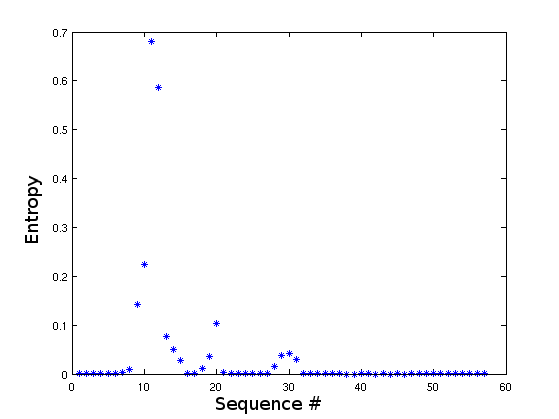
\includegraphics[width=0.48\textwidth]{images/ent_dist1.png}
		\label{fig:ent_dist}
		\caption{Typical entropy distribution for a document in \sysName} 
\end{figure}

where the $p_{j}$ is the marginal probability of label $j$ being the correct label.  Marginal probabilities are calculated using the CRF-variant of the Forward-Backward algorithm \cite{}.  The marginal entropy provides a formulation for a token's individual certainty or uncertainty in its label.  Compare the distributions in Figure~\ref{}.  When the distribution is fairly peaked and we are certain of an answer, the entropy tends to be fairly low.  A more uniform distribution, however, leads to a higher entropy.

\subsection{Reducing the Space of Questions}
\subsubsection{Constraining Tokens Per Document}
While we may sort all of the tokens in the database by entropy and select the top-k, this may lead to less than optimal results.  Individual tokens are not independent.  Modifying the probabilistic label attribute of one token in a document may invoke additional corrections when the inference algorithm is re-run.  We discuss this constrained inference idea further in the context of data integration in Section~\ref{}.  Suffice to say, because we can't anticipate the expected gain from each individual token, we choose not to risk the redundancy of batching multiple high entropy tokens from the same document.

The motivation for this choice can be found in Fig~\ref{fig:ent_dist}, which shows the entropy distribution for a typical document.  The highest entropy values appear in isolated neighborhoods which correspond to the segmentation boundaries.  Since constrained inference primarily supplies additional correction the neighborhoods of constrained tokens, the probability of two selected tokens sharing the same "correction window" is high.  

Thus the strategy implemented is to select only a single token from each document, that token being the one with the highest entropy.  The explicit process can be found in Figure~\ref{} and uses a simple hash map with a docID key to assert only one token per docID is allowed.  All tokens are cycled through in a linear fashion.  If the current docID is not represented in the map, we add it, while if it is represented we only add it if it's entropy is higher than the token currently in the map.  With each document being associated with its highest entropy token, for the remainder of this discussion we refer to selection of a token and selection of document interchangeably.

The existence of such a "correction window" as mentioned above brings up an interesting tradeoff that should be considered.  When the two differ, is it better to select a single highly uncertain token or a token at the center of a high entropy neighborhood, none of whose entropy is as high as the first?  As an additional entropy metric for selection, we introduce the concept of "neighborhood entropy", that is the entropy associated with a token and its nearest neighbors.  It represents a balance between the per-token uncertainty and the expected benefit of crowdsourced answer to its neighbors.  We compare both entropy metrics in the experiments of this paper. 

\begin{figure}
		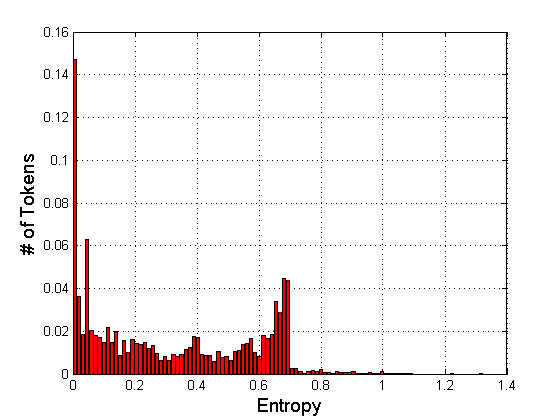
\includegraphics[width=0.48\textwidth]{images/red.png}
		\label{fig:cluster}
		\caption{PLACEHOLDER.} 
\end{figure}

\subsubsection{Clustering Similar Tokens}
Individual documents, especially citation data, may contain significant overlap between authors, conferences, publishers, etc. that appear in more than one document.  While we accept a certain redundancy for quality control purposes, this should be tightly controlled through the AMT interface.  Selecting the same tokens with the same labels from different documents essentially doubles the cost for a single answer.

Our solution to this problem is through a novel clustering technique.  Tokens that share similar text and machine labeling properties have a high probability of sharing the same true labels.  By mapping multiple tokens into the same \textit{Question Cluster}, a single answer can be used to modify labels for a large number of tokens.  Whereas before we constrained the token space to the set of documents, here we constrain the space even further to only the set of unique clusters.  In the rest of this section we describe three specific cluster sets of cluster properties.

All cluster sets require tokens belonging to the cluster to share the same token text and machine labeling, but are set apart by different neighborhood constraints.  Context is important because it's possible that two tokens with the same text such as the word "computer" could actually require different labelings and it would be false to cluster them together.  The different cluster properties trade off accuracy and cluster size and we compare them in the experiments section.  Figure~\ref{fig:cluster} compares two similar tokens and illustrates the different cluster properties that are checked.

\textbf{Same Field:} The strictest of the cluster properties.  It promotes the least amount of clustering, but contains greatest accuracy.  The initial cluster representative defines a field by its CRF max likelihood label and all preceeding and suceeding tokens with the same label.  Tokens are only added to the cluster if they share the entire field.

\textbf{Same Label Neighbhorhood:} A relaxing of the Same Field properties to only compare labels one position before and after the token.  The existence of sub-entities such as a city that appears in more than one Proceedings field or an author that appears with different groups of authors motivate this approach of not checking the entire field.  Clustering is greatly increased, but at the expense of a small amount of misclassification.

\textbf{Same Token Neighborhood:} The simplest of the cluster properties.  We don't check any of the machine labelings, but measure redundancy based purely on the text associated with each token.  Tokens are clustered together that share the same token as well as the same token directly preceeding and suceeding it.  This has the advantage of being purely dependent on the data and not at all on the CRF output.

\sean{One paragraph about implementation of pseudo-code as database procedures somewhere.}

\subsection{Ordering Questions}

The result of running one of the above clustering algorithms reduces the selection problem into one of selecting the \textit{cluster} which provides the maximum reduction of uncertainty in the database.  We consider three different ways of ranking clusters for top-k selection.  Adhering to our information theoretic framework, it's possible to select the "representative" high entropy token used to initiate each cluster and rank by that token's individual entropy.  On the other hand, if clusters are largely skewed in size, it may be more beneficial to rank by the actual size of the cluster.  As a final heuristic attempting to combine both the entropy and cluster size approaches, we can sort by the total entropy of each cluster, that is, the sum of entropies of every token in the cluster.  Our experiments compare and contrast these different ordering techniques. 
